\begin{enumerate}
\item \textbf{Definition} Find $\sin \theta, \cos \theta, \tan \theta$ of the following triangles.
\begin{tasks}[after-item-skip = 30pt, after-skip = 30pt](3)
\task 

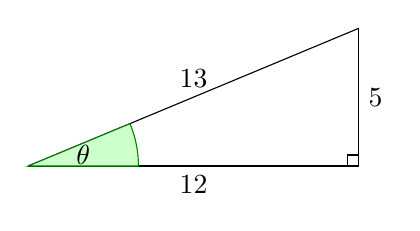
\begin{tikzpicture}[scale=0.7]
\draw (0,0) -- (6,0) node[pos=0.5, below] {12};
\draw (6,0) -- (6,2.5) node[pos=0.5, right] {5};
\draw (6,2.5) -- (0,0) node[pos=0.5, above] {13};
 \filldraw[fill=green!20!white, draw=green!50!black] (0,0) -- (20mm,0mm)
    arc [start angle=0, end angle=22.6, radius=20mm] -- cycle;
\draw (5.8,0) rectangle (6,0.2);
\node[black] at (1,0.2) {$\theta$};
\end{tikzpicture}


\task 

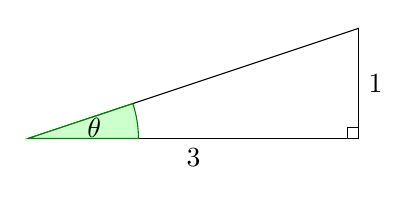
\begin{tikzpicture}[scale=0.7]
\draw (0,0) -- (6,0) node[pos=0.5, below] {3};
\draw (6,0) -- (6,2) node[pos=0.5, right] {1};
\draw (6,2) -- (0,0);
 \filldraw[fill=green!20!white, draw=green!50!black] (0,0) -- (20mm,0mm)
    arc [start angle=0, end angle=18.4, radius=20mm] -- cycle;
\draw (5.8,0) rectangle (6,0.2);
\node[black] at (1.2,0.2) {$\theta$};
\end{tikzpicture}

\task 

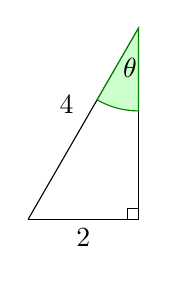
\begin{tikzpicture}[scale=0.7]
\draw (0,0) -- (2,0) node[pos=0.5, below] {2};
\draw (0,0) -- (60:4) node[pos=0.5, above left] {4};
\draw (2,0) -- (60:4);
 \filldraw[fill=green!20!white, draw=green!50!black] (60:4) --+ (0,-1.5)
    arc [start angle=270, delta angle=-30, radius=1.5cm] -- cycle;
\draw (2,0) rectangle (1.8,0.2);
\node[black] at (56:3.3) {$\theta$};
\end{tikzpicture}
\end{tasks}

\item \textbf{Definition} Solve for the unknown sides of the given triangle.
\begin{tasks}[after-item-skip = 30pt, after-skip = 30pt](3)
\task 

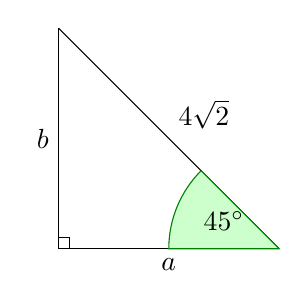
\begin{tikzpicture}[scale=0.7]
\draw (0,0) -- (4,0) node[pos=0.5, below] {$a$};
\draw (0,0) -- (0,4) node[pos=0.5, left] {$b$};
\draw (4,0) -- (0,4) node[pos=0.5, above right] {$4 \sqrt{2}$};
\filldraw[fill=green!20!white, draw=green!50!black] (4,0) -- (2,0)
    arc [start angle=180, delta angle=-45, radius=2cm] -- cycle;
\draw (0,0) rectangle (0.2,0.2);
\node[black] at (3,0.5) {$45^{\circ}$};
\end{tikzpicture}


\task 

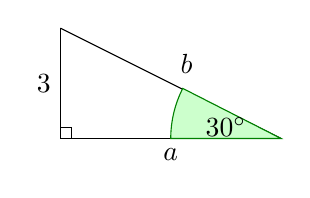
\begin{tikzpicture}[scale=0.7]
\draw (0,0) -- (4,0) node[pos=0.5, below] {$a$};
\draw (0,0) -- (0,2) node[pos=0.5, left] {$3$};
\draw (4,0) -- (0,2) node[pos=0.5, above right] {$b$};
\filldraw[fill=green!20!white, draw=green!50!black] (4,0) -- (2,0)
    arc [start angle=180, delta angle=-27, radius=2cm] -- cycle;
\draw (0,0) rectangle (0.2,0.2);
\node[black] at (3,0.2) {$30^{\circ}$};
\end{tikzpicture}

\task 

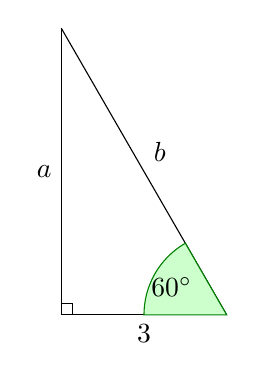
\begin{tikzpicture}[scale=0.7]
\draw (0,0) -- (3,0) node[pos=0.5, below] {$3$};
\draw (0,0) -- (0,5.2) node[pos=0.5, left] {$a$};
\draw (3,0) -- (0,5.2) node[pos=0.5, above right] {$b$};
\filldraw[fill=green!20!white, draw=green!50!black] (3,0) -- (1.5,0)
    arc [start angle=180, delta angle=-60, radius=1.5cm] -- cycle;
\draw (0,0) rectangle (0.2,0.2);
\node[black] at (2,0.5) {$60^{\circ}$};
\end{tikzpicture}
\end{tasks}


\item \textbf{The Unit Circle} Let $\theta$ be the angel such that $0 < \theta < 90^{\circ}$, $\sin \theta = \frac{7}{25}$ and $\cos \theta = \frac{24}{25}$. Draw the unit circle with angels corresponding to the following expressions and compute them.
\begin{tasks}[after-item-skip = 100pt, after-skip = 100pt](2)
\task $\sin(90^{\circ} - \theta)$ and $\cos(90^{\circ}-\theta)$
\task $\sin (90^{\circ} + \theta)$ and $\cos (90^{\circ} + \theta)$
\task $\sin (- \theta)$ and $\cos (- \theta)$
\task $\tan (90^{\circ} - \theta)$ and $\tan (90^{\circ} + \theta)$
\end{tasks}

\newpage

\item \textbf{Trigonometry Identities} 

\begin{tasks}(1)
\task Given that $\sin \alpha = \frac{1}{4}$ for some angle $\alpha$, find $\cos \alpha$.
\vspace{60pt}
\task Given the identity $\cos (2\theta) = 1-2\sin^2 (\theta)$ and the value $\sin (45^\circ) = \frac{\sqrt{2}}{2}$, find $\cos 90^{\circ}$.
\vspace{60pt}
\task Given the identity $\sin (2\theta) = 2\sin (\theta) \cos (\theta)$ and the value $\sin (150^\circ) = \frac{\sqrt{3}}{2}$, find $\sin (300^{\circ})$.
\vspace{100pt}
\task Plot the graphs of $f(x) = \cos(2x)$ and $g(x) = \cos(x)$. Then, use them to find the solutions of $\cos(2x) = \cos(x)$. Make sure that the angular unit is degree, not radian (which we haven't covered yet).
\vspace{100pt}
\task Use the identity $\cos (2\theta) = 2\cos^2 (\theta)-1$ to find the solutions of $\cos (2\theta) = \cos(\theta)$ for $0 \leq \alpha \leq 360$. You'll need to solve a quadratic eqation where $x=\cos(\theta)$. The solutions should match the problem above.
\vspace{150pt}
\end{tasks}
\end{enumerate}